\section{Simulazione SITL}
\subsection{PID}
\subsubsection{STEP}
\todo[inline]{Tabella dei waypoints}
\begin{figure}
	\centering
	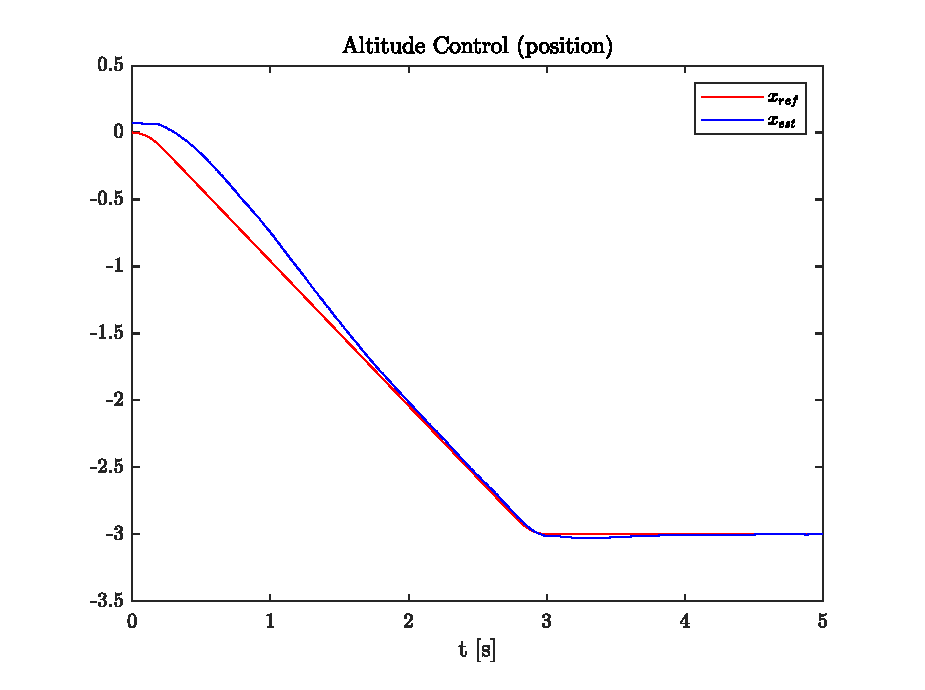
\includegraphics[width=0.5\textwidth]{Simulazioni/Figure/STEPaltitudecontrolposPID}
	\caption{Risposta con PID al segnale STEP : quota}
\end{figure}

\begin{figure}
	\centering
	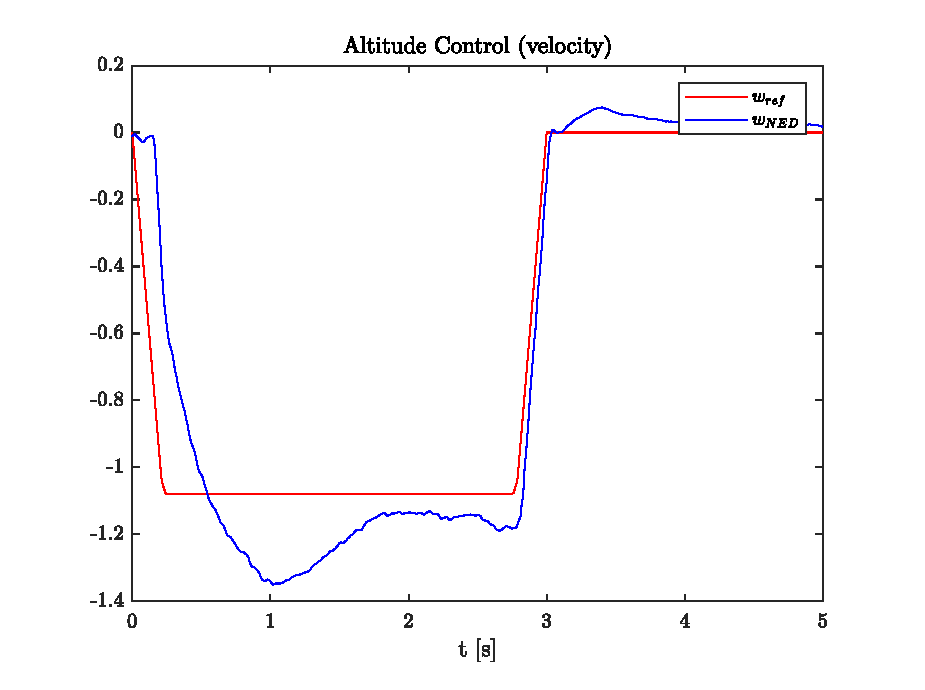
\includegraphics[width=0.5\textwidth]{Simulazioni/Figure/STEPaltitudecontrolvelPID}
	\caption{Risposta con PID al segnale STEP : rateo di salita}
\end{figure}

\begin{figure}
	\centering
	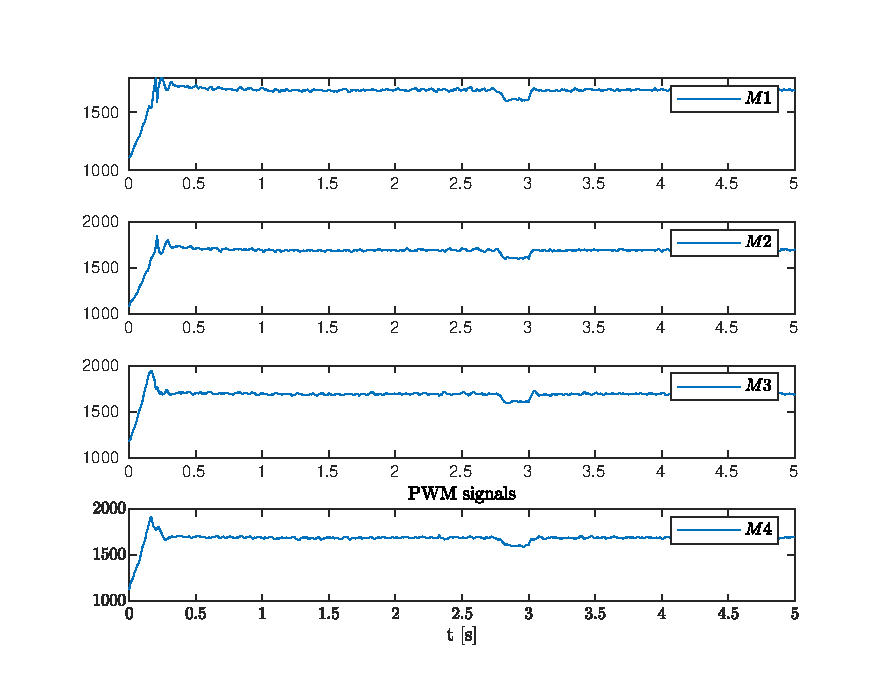
\includegraphics[width=0.5\textwidth]{Simulazioni/Figure/STEPpwmPID}
	\caption{Risposta con PID al segnale STEP : PWM}
\end{figure}

\clearpage
\subsection{SMC}
\subsubsectio{STEP}
\begin{figure}
	\centering
	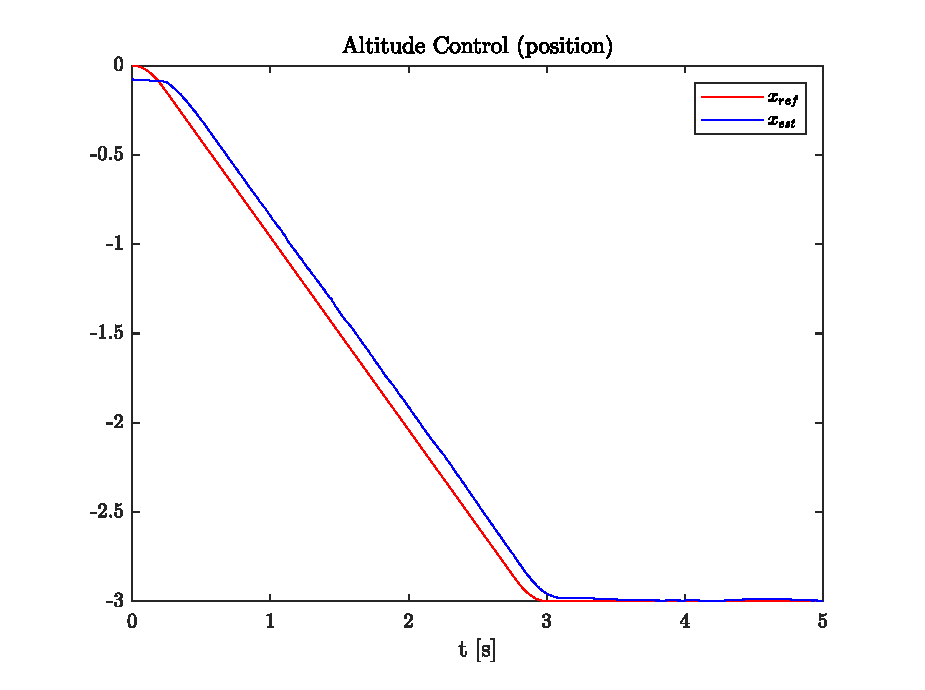
\includegraphics[width=0.5\textwidth]{Simulazioni/Figure/STEPaltitudecontrolposSMC}
	\caption{Risposta con PID al segnale STEP : quota}
\end{figure}

\begin{figure}
	\centering
	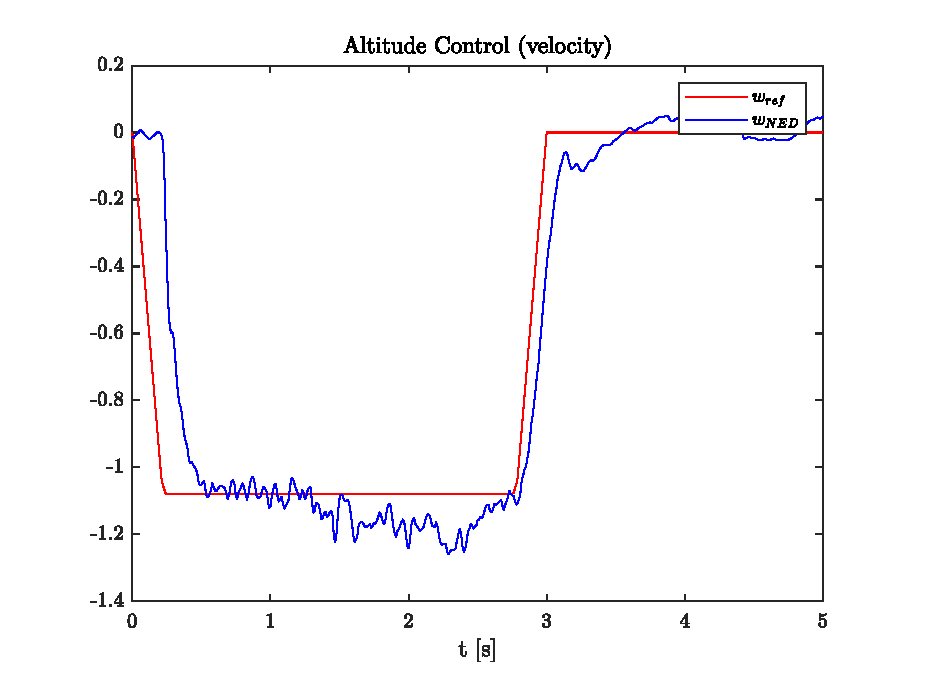
\includegraphics[width=0.5\textwidth]{Simulazioni/Figure/STEPaltitudecontrolvelSMC}
	\caption{Risposta con PID al segnale STEP : rateo di salita}
\end{figure}

\begin{figure}
	\centering
	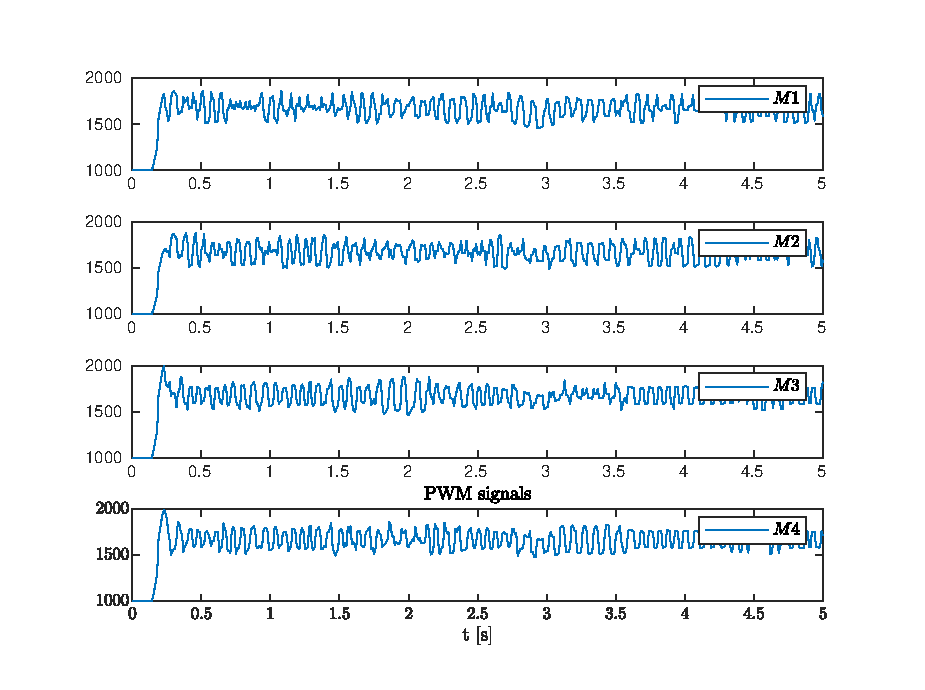
\includegraphics[width=0.5\textwidth]{Simulazioni/Figure/STEPpwmSMC}
	\caption{Risposta con PID al segnale STEP : PWM}
\end{figure}

\clearpage
\subsection{Confronto}